\documentclass[10pt,aspectratio=169]{beamer}
\usepackage{poly}
\usepackage{algorithm}
\usepackage{algorithmic}
\usepackage{listings}
\usepackage{xcolor}

% ================================================================================
% Metadata
% ================================================================================

\title{Westlake Beamer Presentation Theme}
\subtitle{Using \LaTeX\ to prepare slides}
\author{ZX}
\institute[COMP]{School of Engineering}
\date{\today}
\definecolor{codegray}{rgb}{0.95,0.95,0.95}

\lstset{
  backgroundcolor=\color{codegray},
  basicstyle=\ttfamily\footnotesize,
  keywordstyle=\color{blue},
  commentstyle=\color{gray},
  stringstyle=\color{red},
  showstringspaces=false,
  frame=single,
  language=Python
}

% ================================================================================
% Main Body
% ================================================================================

\begin{document}
\maketitle % generate the title slide

\section{Introduction}

\begin{frame}{Slide-Making in \LaTeX}

	We assume that you can use \LaTeX. If not, you can refer to \href{https://www.overleaf.com/learn/latex/Learn_LaTeX_in_30_minutes}{this page}.

	\href{https://www.overleaf.com/learn/latex/Beamer}{Beamer} is one of the most popular and influential document classes for slide-making in \LaTeX. You can find its \href{https://mirror-hk.koddos.net/CTAN/macros/latex/contrib/beamer/doc/beameruserguide.pdf}{full manual here}.

	Here, we will only introduce the basic functionalities so you can master them immediately.
\end{frame}


\begin{frame}{Beamer vs. MS PowerPoint}

	Compared to Microsoft PowerPoint, \LaTeX\ and Beamer provides these advantages:
	
	\begin{itemize}
		\item Beamer produces a \texttt{.pdf} file with no problems on fonts, formulas, or program versions.
		\item Math typesetting in \LaTeX\ is much easier, e.g.,
			\begin{equation*}
				\mathrm{i}\,\hslash\frac{\partial}{\partial t} \Psi(\mathbf{r},t) =
				-\frac{\hslash^2}{2\,m}\nabla^2\Psi(\mathbf{r},t)
				+ V(\mathbf{r})\Psi(\mathbf{r},t).
			\end{equation*}
	\end{itemize}
\end{frame}

\section{Examples}

\begin{frame}[fragile]{Document Class}

	To begin with, just use \texttt{beamer} document class with \texttt{poly} theme. It should be noted that the \texttt{poly.sty} file should be included in the same directory as the \texttt{main.tex} file.
	
\begin{block}{Preamble about the document class}
\begin{lstlisting}[language=TeX]
\documentclass[10pt,aspectratio=169]{beamer}
\usepackage{poly}
\end{lstlisting}
\end{block}
	
	You can change the \texttt{aspectratio} to \texttt{43} to adjust the slide aspect ratio to 4:3.
\end{frame}

\begin{frame}[fragile]{Metadata}
	You can change the metadata displayed on the title slide:

\begin{block}{Metadata}
\begin{lstlisting}[language=TeX]
\title{Your Title}
\subtitle{Your Subtitle}
\author{First Author, Second Author}
\institute[COMP]{Department of Computing}
\date{Date}
\end{lstlisting}
\end{block}

	Once settled, you can render the title slide with the command \verb|\maketitle| in the body.
\end{frame}

\begin{frame}[fragile]{Texts}{In a Sequence}

	\begin{itemize}[<+->]
		\item A typical slide has bulleted points.
		\item These can be uncovered in sequence.
		\item When rendered, they will be separated into multiple slides.
	\end{itemize}

\end{frame}

\begin{frame}{Images}

	Adding images works like in normal \LaTeX:
	
	\begin{figure}[hbt]
		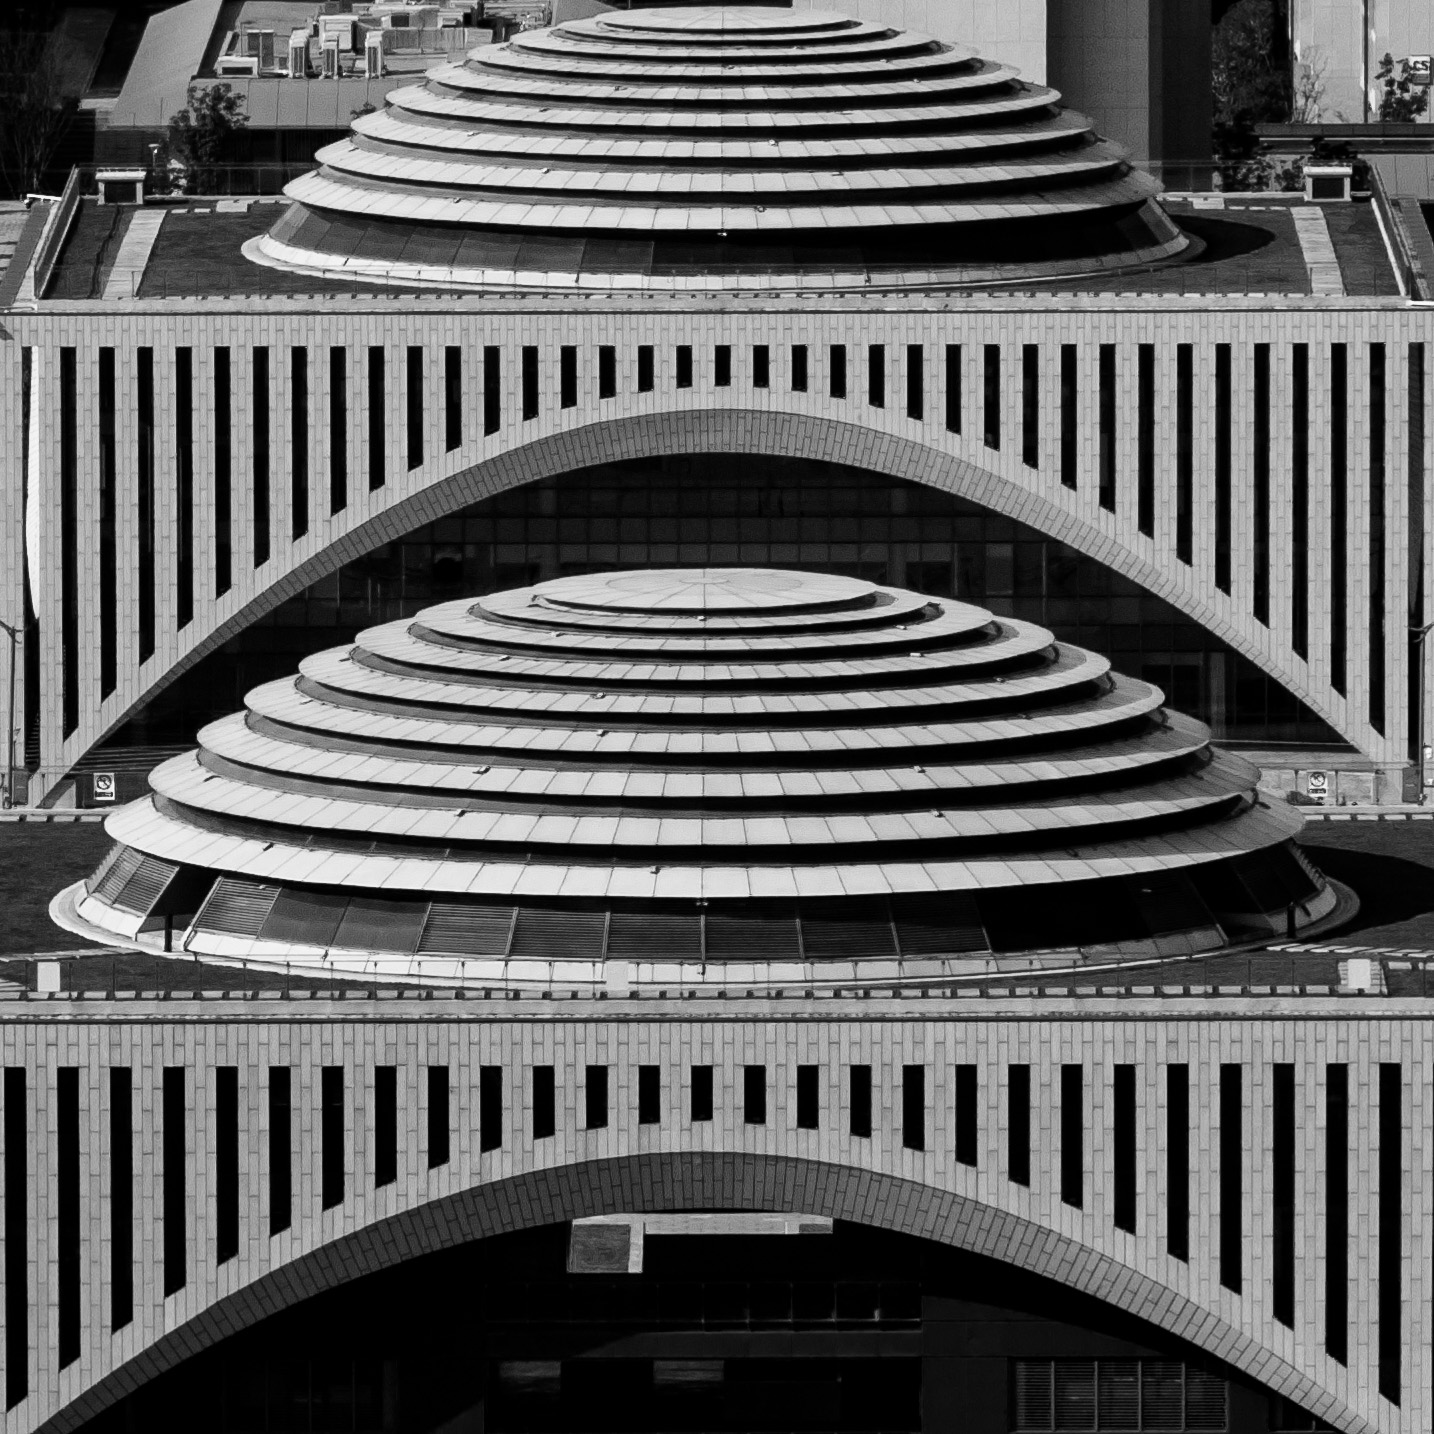
\includegraphics[width=0.3\textwidth]{source/picture3.jpg}
 		\caption{A sample of image}
	\end{figure}
	
\end{frame}

\begin{frame}{Columns}
	Splitting the page is easy and common.

	Typically, one side has a picture and the other text:
	
	\vspace{20pt}
	
	\begin{columns}
		\begin{column}{0.6\textwidth}
			This is the first column.\\[10pt]
			You can have some texts here.
		\end{column}
		
		\begin{column}{0.3\textwidth}
			And this is the second one.\\[10pt]
			You can have some pictures or tables here.
		\end{column}
	\end{columns}

\end{frame}
\begin{frame}[fragile]{Codes}

\begin{lstlisting}
def fibonacci(n):
    if n == 0:
        return 0
    elif n == 1:
        return 1
    a, b = 0, 1
    for _ in range(2, n + 1):
        a, b = b, a + b
    return b
\end{lstlisting}
\end{frame}

\begin{frame}{Fonts}
	
	The priority when choosing a font is readability.
	
	Here, we give some advice:
	\begin{itemize}
		\item Use serif (default) fonts only with high-resolution projectors or monitors.
		\item Use \textsf{sans-serif} fonts otherwise.
		\item Use \textit{italic} or \textbf{bold} fonts to emphasize or highlight points.
		\item We also provide an \alert{alert} font for emphasise.
		\item Use \texttt{monospace} fonts to display codes.
	\end{itemize}

\end{frame}

\section{Summary}

\begin{frame}{Good Luck!}
	\begin{itemize}
		\item Enough for an introduction! You should know enough by now.
		\item If you have corrections or suggestions, please feel free to contact \href{mailto:ruisong20@gmail.com}{me}!
        \item You can also find this project on \href{https://github.com/wurahara/PolyU-Beamer-Slides}{Github}! Stars are welcome!
	\end{itemize}
\end{frame}

\backmatter % generate the final slide
\end{document}
